\documentclass[main.tex]{subfiles}
\begin{document}
\chapter*{Samarbejdsaftale}


Samarbejdsaftale mellem \textbf{Mohamed Hussein Mohamed} og\textbf{ Martin Banasik} i forbindelse med Bachelorprojekt Synkerefleksmonitor på Sundhedsteknologi. 

\subsection*{Daglige arbejde}
Hver morgen kl. 9:00 afholdes et internet scrum møde, for at orientere i gruppen om nuværende opgaver og problemstillinger herom. 
Da gruppen sidder i samme lokale er det muligt at hjælpe hinanden , men samtidig forventes det, at der selv søges hjælp til selvstændige opgaver efter behov. 

\subsection*{Sygdom}
Hvis et gruppe medlem er sygt, skal dette meddeles til gruppen a.s.a.p. og komme med en forventet længde af denne.

\subsection*{Ledelse}
Kollektiv ledelse. 
Alle beslutninger træffes i fællesskab. 
Enkelte mindre beslutninger kan tages af det enkelte individ, så længe parterne har givet godkendelse. 

\subsection*{Arbejdsplads og tid}
Gruppen mødes alle hverdage i lokalet K231 og arbejder til kl. 16:00. Da der bliver fulgt fag ved siden af bachelorprojektet er ikke alle dage der er ens. Se overblik over hele ugen i figur \ref{ugeplan}. Ved spidsbelastninger og deadlines kan weekender og aftener tages i brug.

\subsection*{Møder}
Der indkaldes til vejledermøde en gang ugentlig, hver onsdag kl. 9:00. 
Til hvert møde, laves der en mødeindkaldelse, der indeholder en dagsorden og denne vil blive udsendt senest et døgn før mødet.
Fravær og aflysning af et møde aftales indbyrdes. 
Ved hvert møde er der ansvar for at der skrives et referat og for at være ordstyrer, som går på tur.

\subsection*{Logbog}
Beslutninger, ændringer og større arbejde ifm. projektet noteres i logbogen. 

\subsection*{Ambitionsniveau}
Parterne er enige om at, at yde det bedste. 
 
\subsection*{Misligholdelse af aftaler}
Ved samarbejdsproblemer løser parterne problemerne indbyrdes. 
Ved manglende bidragelse til projektarbejdet inddrages projektvejleder.

 
\subsection*{Roller}
\begin{itemize}
\item Ansvarlig for fysiske dokumenter og organisering af disse er \textbf{Martin}
\item Ansvarlig for logbog er \textbf{Mohamed}
\item Ansvarlig for mødeindkaldelse og mødereferater er \textbf{Mohamed}
\item{Hardware}
\item{Software}
\end{itemize}

\begin{figure}[H]
\centering
{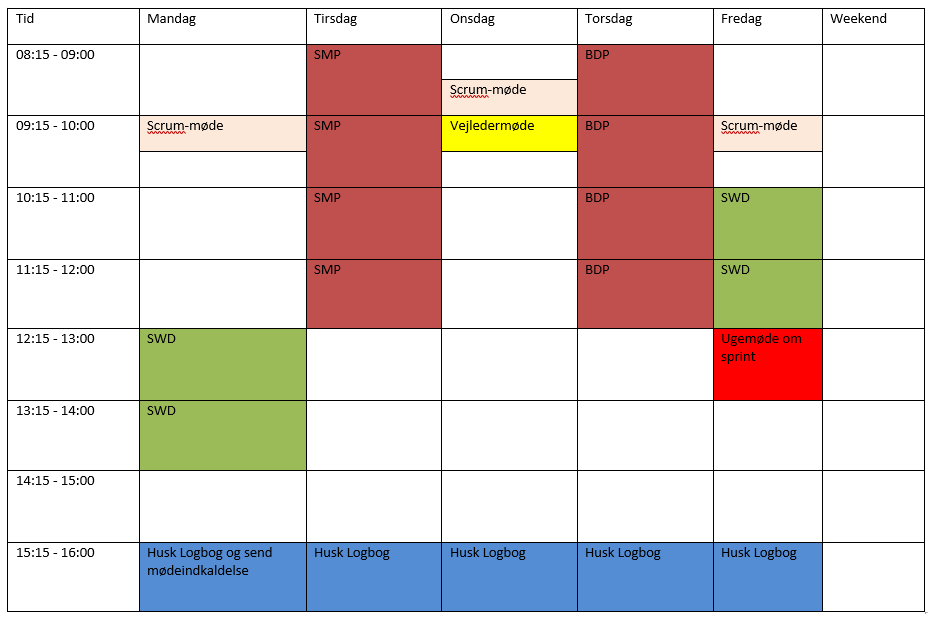
\includegraphics[width=16cm]
{Figure/Ugeplan}}
\caption{Ugeskema med faste mødetider og aftaler i løbet af ugen.}
\label{ugeplan}
\end{figure}

\newpage
Med nedenstående underskrifter bekræfter hver partener, at de har godkendt kontrakten, står inde for den og vil overholde den. 
 
Underskrifter:

\begin{vplace}[0.1]

\noindent \begin{tabular}{ll}

\includegraphics[height=1cm]{Figure/underskriftmohamed} & 
\includegraphics[height=1cm]{Figure/underskriftdato}\\
	\makebox[3in]{\hrulefill} & \makebox[1.5in]{\hrulefill}\\
	Mohamed Hussein Mohamed  (201370525) & Dato\\[9ex]
    
\includegraphics[height=1cm]{Figure/underskriftmartin} & 
\includegraphics[height=1cm]{Figure/underskriftdato} \\
	\makebox[3in]{\hrulefill} & \makebox[1.5in]{\hrulefill}\\
	Martin Banasik  (201408398) & Dato\\[7ex]
		
\end{tabular}

\end{vplace}

\end{document}